% Source-derived chapter 13: Elimination of \texorpdfstring{$\I_4^*$}{I4*}-fibers
% Original source: no-enriques-surface-over-the-integers
\chapter{Elimination of \texorpdfstring{$\I_4^*$}{I4*}-fibers}
\label{no-enriques-surface-over-the-integers-chapter-13}
\source{no-enriques-surface-over-the-integers}

\begin{remark}[Source section]
\label{no-enriques-surface-over-the-integers-chapter-13-source}
\source{no-enriques-surface-over-the-integers}
\source{no-enriques-surface-over-the-integers}
This chapter reproduces the corresponding section of the retrieved
LaTeX source, including its definitions, statements, examples, and
proofs. It has not yet been translated into Lean.
\notready
\end{remark}

% The source section title was: Elimination of \texorpdfstring{$\I_4^*$}{I4*}-fibers
\mylabel{Elimination I4*}

Let $Y$ be a non-exceptional Enriques surface over the ground field $k=\FF_2$,  with constant Picard scheme.
The goal of this section is   to exclude the two $\I_4^*$-cases from the table in Proposition \ref{key reduction}.

\begin{proposition}
\source{no-enriques-surface-over-the-integers}
\notready
\mylabel{no I4*}
There is no genus-one fibration 
$\varphi:Y\ra\PP^1$ having a fiber  with Kodaira symbol $\I_4^*$. 
\end{proposition}

\proof
Seeking a contradiction, we assume that $\varphi^{-1}(\infty)$ has Kodaira symbol $\I_4^*$. Its dual graph is:
\begin{equation*}
% dual graph I4*
\begin{gathered}
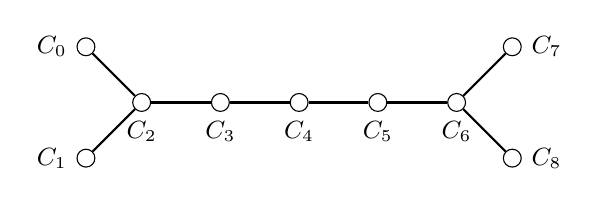
\begin{tikzpicture}
[node distance=1cm, font=\small]
\tikzstyle{vertex}=[circle, draw, fill=white, inner sep=0mm, minimum size=1.5ex]
\node[vertex]	(C2)  	at (1,0) 	[label=below:{$C_2$}] 		{};
\node[vertex]	(C3)			[right of=C2, label=below:{$C_3$}]	{};
\node[vertex]	(C4)			[right of=C3, label=below:{$C_4$}]	{};
\node[vertex]	(C5)			[right of=C4, label=below:{$C_5$}]	{};
\node[vertex]	(C6)			[right of=C5, label=below:{$C_6$}]	{};

\node[vertex]	(C7)			[above right of=C6, label=right:{$C_7$}]	{};
\node[vertex]	(C8)			[below right of=C6, label=right:{$C_8$}]	{};
\node[vertex]	(C0)			[above left  of=C2, label=left :{$C_0$}]	{};
\node[vertex]	(C1)			[below left  of=C2, label=left :{$C_1$}]	{};

\draw [thick] (C2)--(C3)--(C4)--(C5)--(C6);
\draw [thick] (C0)--(C2)--(C1);
\draw [thick] (C7)--(C6)--(C8);
\end{tikzpicture}
\end{gathered}
\end{equation*}
The fiber must be simple, according to   Proposition \ref{key reduction}, 
so the schematic fiber is  $\varphi^{-1}(\infty) = C_0+C_1+2(C_2+\ldots+C_6)+C_7+C_8$.
Moreover,  there is a genus-one fibration $\psi:Y\ra\PP^1$ so that the multiple fiber $2F$ have  $F\cdot\varphi^{-1}(\infty)=2$.
After renumeration, we have the following   possibilities: $(F\cdot C_i)=1$ with $i\in\{2,3,4\}$
or $(F\cdot C_0)=(F\cdot C_1)=1$ or $(F\cdot C_0)=(F\cdot C_8)=1$ or $(F\cdot C_0)=2$.
Our task is to rule out each of these six possibilities. 
Without restriction, we assume that   $\psi^{-1}(\infty)$ contains the largest number of irreducible components
among all fibers.

Suppose first that $(F\cdot C_4)=1$. Then the connected curves $C_0+\ldots+C_3$ and $C_5+\ldots+C_8$ both have
dual graph $T_{2,2,2}$ and are contained in some fibers of $\psi$. According to Proposition \ref{key reduction}, 
they both must be contained in  
$\psi^{-1}(\infty)$, which therefore has  Kodaira symbol $\I_4^*$ and must be simple.
Let $R\subset \psi^{-1}(\infty)$ the additional component, which has $(R\cdot C_i)=(R\cdot C_j)=1$ for some
$i\in\{0,1,3\}$ and $j\in\{5,7,8\}$. Let $1\leq m_i,m_j\leq 2$ be the multiplicities of $C_i,C_j\subset\varphi^{-1}(\infty)$.
From
$$
4=\varphi^{-1}(\infty)\cdot\psi^{-1}(\infty) = (m_iC_i+2C_4+m_jC_j)\cdot 2R = 2m_i+4(C_4\cdot R) + 2m_j 
$$
we infer that $R\cap C_4=\varnothing$ and $m_i=m_j=1$. After renumeration,
we may assume $i=1$ and $j=7$. Then $C_1+\ldots+C_7+R$ is a curve
of canonical type $\I_8$, in contradiction to Proposition \ref{key reduction}.

Suppose next that $(F\cdot C_3)=1$.  
The connected curve $C_4+\ldots+C_8$ has dual graph $T_{2,2,3}$ and must be contained in   $\psi^{-1}(\infty)$.
The curve $C_0+C_2+C_1$ is a chain and must be part of some fiber $\psi^{-1}(t)$ as well.
If $t\neq\infty$, 
we infer from Proposition \ref{key reduction} that $\psi^{-1}(t)$ has Kodaira symbol $\I_4$ 
and is simple.  Let $R\subset \psi^{-1}(t)$ be the additional component, with $(R\cdot C_0)=(R\cdot C_1)=1$.
This gives 
$$
4=\varphi^{-1}(\infty)\cdot \psi^{-1}(t) = (C_0+C_1+2C_3) \cdot R = 1+1+ 2(C_3\cdot R),
$$
and hence  $(C_3\cdot R)=1$. Thus $C_1+C_2+C_3+R$ is another curve of canonical type $\I_4$. Its intersection number with $C_4$ is one,
so the fiber is multiple, contradiction.
Summing up,  $C_0+C_1+C_2$ and $C_4+\ldots+C_8$ both belong to   $\psi^{-1}(\infty)$, which therefore
has Kodaira symbol $\I_4^*$ and must be simple, in light of Proposition \ref{key reduction}. Let $R$ be the additional component, which necessarily has
$(R\cdot C_2)=(R\cdot C_4)=1$. This gives 
$$
4=\varphi^{-1}(\infty)\cdot \psi^{-1}(\infty) = (2C_2+2C_3+2C_4)\cdot 2R = 4+4(C_3\cdot R) + 4\geq 8,
$$
contradiction.

Now suppose that $(F\cdot C_2)=1$. Then the connected curve $C_3+\ldots + C_8$ has dual graph $T_{2,2,4}$ 
and must be contained in $\psi^{-1}(\infty)$. Its Kodaira symbol is either $\II^*$, $\I_4^*$, $\III^*$ or $\I_2^*$.
The first alternative  is impossible by Proposition \ref{key reduction}. 
In the second alternative, the fiber must be simple.
The additional component $R\subset\psi^{-1}(\infty)$ has $(R\cdot C_i)=1$ for all $i\in\{0,1,3\}$,
which gives the contradiction
$$
4=\varphi^{-1}(\infty)\cdot\psi^{-1}(\infty) = (C_0+C_1+2C_2+2C_3)\cdot 2R= 2+2+4(C_2\cdot R) + 4\geq 8.
$$
In the third  alternative, we deduce
from Proposition \ref{key reduction} that one of the curves from $C_0+C_1$ also belongs to $\psi^{-1}(\infty)$.
Without restriction, we may assume that this is $C_1$. Let $R\subset\psi^{-1}(\infty)$ be the additional component,
say with  $(R\cdot C_7)=(R\cdot C_1)=1$. From
$$
4\geq \varphi^{-1}(\infty)\cdot\psi^{-1}_\ind(\infty) = (C_1+2C_2+C_7)\cdot 2R = 2+ 4(C_2\cdot R) + 2
$$
we get $R\cap  C_2=\varnothing$. But then $C_1+\ldots+C_7+R$ is a curve of canonical type $\I_8$, in contradiction
to Proposition \ref{key reduction}.
The only remaining possibility is that  $\psi^{-1}(\infty) $ has Kodaira symbol $\I_2^*$.
So the additional component $R\subset\psi^{-1}(\infty)$ has $(R\cdot C_4)=1$. From
$$
4\geq \varphi^{-1}(\infty)\cdot\psi^{-1}_\ind(\infty) = (2C_2+2C_4)\cdot R=   2(C_2\cdot R) + 2
$$
we deduce that $(C_2\cdot R)$ is either zero or one.
In the latter case we get a curve $D=C_2+C_3+C_4+R$ of canonical type $\I_4$.
The ensuing fiber is multiple, because $(D\cdot C_5)=1$, in contradiction to Proposition \ref{key reduction}.
The former case yields the following dual graph, in contradiction to  Proposition \ref{no I4*+R} below.
\begin{equation*}
\begin{gathered}
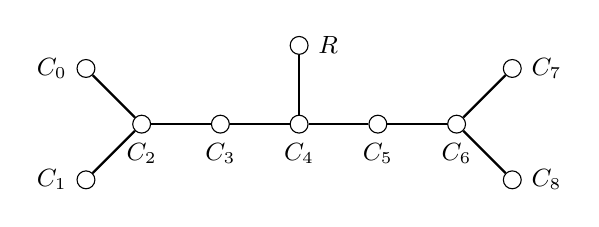
\begin{tikzpicture}
[node distance=1cm, font=\small]

\tikzstyle{vertex}=[circle, draw, fill=white, inner sep=0mm, minimum size=1.5ex]
\node[vertex]	(C2)  	at (1,0) 	[label=below:{$C_2$}] 		{};
\node[vertex]	(C3)			[right of=C2, label=below:{$C_3$}]	{};
\node[vertex]	(C4)			[right of=C3, label=below:{$C_4$}]	{};
\node[vertex]	(C5)			[right of=C4, label=below:{$C_5$}]	{};
\node[vertex]	(C6)			[right of=C5, label=below:{$C_6$}]	{};

\node[vertex]	(C7)			[above right of=C6, label=right:{$C_7$}]	{};
\node[vertex]	(C8)			[below right of=C6, label=right:{$C_8$}]	{};
\node[vertex]	(C0)			[above left  of=C2, label=left :{$C_0$}]	{};
\node[vertex]	(C1)			[below left  of=C2, label=left :{$C_1$}]	{};
\node[vertex]	(R)			[above of=C4, label=right :{$R$}]	{};

\draw [thick] (C2)--(C3)--(C4)--(C5)--(C6);
\draw [thick] (C0)--(C2)--(C1);
\draw [thick] (C7)--(C6)--(C8);
\draw [thick] (C4)--(R);
\end{tikzpicture}
\end{gathered}
\end{equation*}
Next, suppose that we are in the case $(F\cdot C_0)=(F\cdot C_1)=1$. Then the connected curve $C_2+\ldots+C_8$
has dual graph $T_{2,2,5}$  and must be contained in $\psi^{-1}(\infty)$.
The possible Kodaira symbols are $\II^*$ and $\I_4^*$. 
The former is impossible by Proposition \ref{key reduction}, so $\psi^\inv(\infty)$ is simple with Kodaira symbol $\I_4^*$.   
Let $R,R'\subset\psi^{-1}(\infty)$ be the two additional components,
with $(R\cdot C_2)=(R'\cdot C_2)=1$. Then $4=\varphi^{-1}(\infty)\cdot \psi^{-1}(\infty)$ becomes
$$
(C_0+C_1+2C_2)\cdot (R+R') = (C_0+C_1)\cdot (R+R') + 2+2, 
$$
and we infer that $R\cup R'$ is disjoint from $C_0\cup C_1$. In turn, $C_0+C_1+R+R'+C_2$ supports a curve of canonical type
$\I_0^*$, in  contradiction to Proposition \ref{key reduction}.

Now suppose $(F\cdot C_0)=(F\cdot C_8)=1$. Then $C_1+\ldots +C_7$ is a chain and contained in $\psi^{-1}(\infty)$.
The possible Kodaira symbols are $\I_4^*$ or $\III^*$, by Proposition \ref{key reduction}. 
The symbol $\I_4^*$ is handled as in the preceding paragraph. In the remaining case $\III^*$, let $R\subset \psi^{-1}(\infty)$ be the
additional component, which has $(R\cdot C_4)=1$. From
$$
4\geq \varphi^{-1}(\infty)\cdot \psi^{-1}_\ind(\infty) = (C_0+2C_4+C_8)\cdot 2R = 2(C_0\cdot R) + 4 + 2(C_8\cdot R)
$$
we infer that $R$ is disjoint from $C_0\cup C_8$. Now the configuration $C_0+\ldots+C_8+R$ contradicts Proposition \ref{no I4*+R} below.

It remains to cope with the last possibility   $(F\cdot C_0)=2$, which is the most difficult. 
Now the connected curve $C_1+\ldots+C_8$ has dual graph $T_{2,2,6}$
and must be contained in $\psi^{-1}(\infty)$. Its Kodaira symbol has to be $\I_4^*$, so the fiber is simple. The additional
component $R\subset\psi^{-1}(\infty)$ has $(R\cdot C_2)=1$, and from
$$
4=\varphi^\inv(\infty)\cdot \psi^\inv(\infty) = (C_0+2C_2)\cdot R = (C_0\cdot R) + 2
$$
we infer that the dual graph for $C_0+\ldots+C_8+R$ must be:
\begin{equation*}
% dual graph I4*
\begin{gathered}
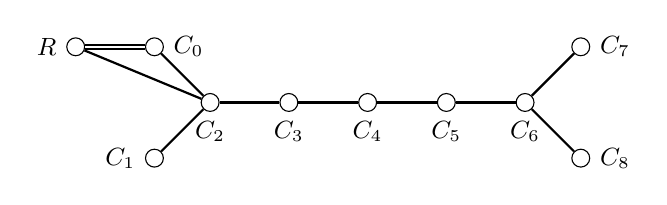
\begin{tikzpicture}
[node distance=1cm, font=\small]
\tikzstyle{vertex}=[circle, draw, fill=white, inner sep=0mm, minimum size=1.5ex]
\node[vertex]	(C2)  	at (1,0) 	[label=below:{$C_2$}] 		{};
\node[vertex]	(C3)			[right of=C2, label=below:{$C_3$}]	{};
\node[vertex]	(C4)			[right of=C3, label=below:{$C_4$}]	{};
\node[vertex]	(C5)			[right of=C4, label=below:{$C_5$}]	{};
\node[vertex]	(C6)			[right of=C5, label=below:{$C_6$}]	{};

\node[vertex]	(C7)			[above right of=C6, label=right:{$C_7$}]	{};
\node[vertex]	(C8)			[below right of=C6, label=right:{$C_8$}]	{};
\node[vertex]	(C0)			[above left  of=C2, label=right :{$C_0$}]	{};
\node[vertex]	(C1)			[below left  of=C2, label=left :{$C_1$}]	{};
\node[vertex]	(R)				[left of=C0, label=left :{$R$}]	{};

\draw [thick] (C2)--(C3)--(C4)--(C5)--(C6);
\draw [thick] (C0)--(C2)--(C1);
\draw [thick] (C7)--(C6)--(C8);
\draw [thick, double] (C0)--(R);
\draw [thick] (C2)--(R);
\end{tikzpicture}
\end{gathered}
\end{equation*}
%\emph{Here the double edge indicates that the   scheme $C_0\cap C'_0$ has length two}.
But this configuration is impossible, by Proposition \ref{no I4*+R second} below.
\qed

\medskip
In the above arguments, we have used the following facts:

\begin{proposition}
\source{no-enriques-surface-over-the-integers}
\notready
\mylabel{no I4*+R}
There is no configuration $C_0+\ldots+C_8+R$ of ten $(-2)$-curves on $Y$ with simple normal crossings and the following dual graph:
\begin{equation}
\label{I4*+R}
\source{no-enriques-surface-over-the-integers}
\begin{gathered}
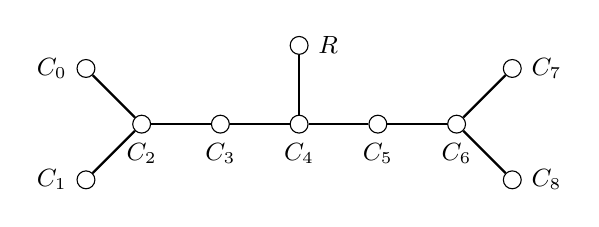
\begin{tikzpicture}
[node distance=1cm, font=\small]

\tikzstyle{vertex}=[circle, draw, fill=white, inner sep=0mm, minimum size=1.5ex]
\node[vertex]	(C2)  	at (1,0) 	[label=below:{$C_2$}] 		{};
\node[vertex]	(C3)			[right of=C2, label=below:{$C_3$}]	{};
\node[vertex]	(C4)			[right of=C3, label=below:{$C_4$}]	{};
\node[vertex]	(C5)			[right of=C4, label=below:{$C_5$}]	{};
\node[vertex]	(C6)			[right of=C5, label=below:{$C_6$}]	{};

\node[vertex]	(C7)			[above right of=C6, label=right:{$C_7$}]	{};
\node[vertex]	(C8)			[below right of=C6, label=right:{$C_8$}]	{};
\node[vertex]	(C0)			[above left  of=C2, label=left :{$C_0$}]	{};
\node[vertex]	(C1)			[below left  of=C2, label=left :{$C_1$}]	{};
\node[vertex]	(R)			[above of=C4, label=right :{$R$}]	{};

\draw [thick] (C2)--(C3)--(C4)--(C5)--(C6);
\draw [thick] (C0)--(C2)--(C1);
\draw [thick] (C7)--(C6)--(C8);
\draw [thick] (C4)--(R);
\end{tikzpicture}
\end{gathered}
\end{equation}
\end{proposition}

\proof
Seeking a contradiction, we assume that the configuration  exists. 
The subconfiguration  $C_0+\ldots+C_8$ supports a curve of canonical type $\I_4^*$. Let $\varphi:Y\ra\PP^1$ be the resulting
genus-one fibration.  Without restriction, we may assume that 
$\varphi^{-1}(\infty) = C_0+C_1+2(C_2+\ldots+C_6)+C_7+C_8$.
The fiber   indeed must be simple by Proposition \ref{key reduction}. Write $F\subset Y$ for some half-fiber, and let 
$S\subset\Num(Y)$ be the subgroup generated by $C_1,\ldots,C_8,R,F$.
To proceed, we exploit properties of the resulting Gram matrix $N\in\Mat_{10}(\ZZ)$, which can easily be checked
with computer algebra.
% with computer algebra, for example \cite{Magma}.
One computes in this way $\det(N)=-4$, whence $S\subset \Num(Y)$ if a subgroup of index two.
% /*
%        9
%        |
%    2-3-4-5-6-7
%    |       |
%    1       8
%    R= two-section = ninth basis vector
%    F= half-fiber  = tenth basis vector
% */
% 
% 
% Q:=RationalField();
% Z:=IntegerRing();
% 
% N:=ScalarMatrix(10,Q!-2); N[10,10]:=0;
% for i:= 1 to 6 do
% N[i,i+1]:=1; N[i+1,i]:=1;
% end for;
% N[8,6]:=1; N[6,8]:=1;
% N[9,4]:=1; N[4,9]:=1;
% N[10,9]:=1; N[9,10]:=1;
% 
% N; Determinant(N); pSignature(N,-1);
% [-2  1  0  0  0  0  0  0  0  0]
% [ 1 -2  1  0  0  0  0  0  0  0]
% [ 0  1 -2  1  0  0  0  0  0  0]
% [ 0  0  1 -2  1  0  0  0  1  0]
% [ 0  0  0  1 -2  1  0  0  0  0]
% [ 0  0  0  0  1 -2  1  1  0  0]
% [ 0  0  0  0  0  1 -2  0  0  0]
% [ 0  0  0  0  0  1  0 -2  0  0]
% [ 0  0  0  1  0  0  0  0 -2  1]
% [ 0  0  0  0  0  0  0  0  1  0]
% -4
% -8

Nikulin's theory of discriminant forms \cite{Nikulin 1980} allows us to use the lattice $S$ to gain enough control of the slightly larger  $\Num(Y)$
and thus the geometry of  $Y$.
Set $S^*=\Hom(S,\ZZ)$, and consider the   injection $ S\ra S^*$ given by $x\mapsto (y\mapsto (x\cdot y))$.
This linear map is described, with respect to the given basis $C_1,\ldots,F\in S$ and the   dual basis $C_1^*,\ldots,F^*\in S^*$, 
by the matrix    $N\in\Mat_n(\ZZ)$.
With respect to this dual basis, the  induced $\QQ$-valued form   on $S^*$ has Gram matrix 
\begin{equation}
\label{gram matrix}
\source{no-enriques-surface-over-the-integers}
N^{-1}=
{\tiny
\begin{pmatrix} 
  -1   &-1   &-1   &-1   &-1   &-1 &-1/2 &-1/2   & 0   & 1\\
  -1   &-2   &-2   &-2   &-2   &-2  & -1 &  -1   & 0   & 2\\
  -1   &-2   &-3   &-3   &-3   &-3 &-3/2 &-3/2   & 0   & 3\\
  -1   &-2   &-3   &-4  & -4   &-4 &  -2 &  -2   & 0   & 4\\
  -1   &-2   &-3   &-4   &-5   &-5 &-5/2 &-5/2   & 0   & 4\\
  -1   &-2   &-3   &-4   &-5   &-6 &  -3 &  -3   & 0   & 4\\
-1/2   &-1 &-3/2   &-2 &-5/2   &-3 &  -2 &-3/2   & 0   & 2\\
-1/2   &-1 &-3/2   &-2 &-5/2   &-3 &-3/2 &  -2   & 0   & 2\\
   0   & 0   & 0   & 0  &  0   & 0 &   0 &   0   & 0   & 1\\
   1   & 2   & 3   & 4  & 4    &4  &  2  &  2    & 1   &-2
\end{pmatrix}
}
\end{equation}
and we have $S\subset\Num(Y)\subset S^*$.  Note that for each  column, the entries are the coordinates of the corresponding
dual basis vectors with respect to the basis vectors.
%
% S:=N^-1;
% S;
% [  -1   -1   -1   -1   -1   -1 -1/2 -1/2    0    1]
% [  -1   -2   -2   -2   -2   -2   -1   -1    0    2]
% [  -1   -2   -3   -3   -3   -3 -3/2 -3/2    0    3]
% [  -1   -2   -3   -4   -4   -4   -2   -2    0    4]
% [  -1   -2   -3   -4   -5   -5 -5/2 -5/2    0    4]
% [  -1   -2   -3   -4   -5   -6   -3   -3    0    4]
% [-1/2   -1 -3/2   -2 -5/2   -3   -2 -3/2    0    2]
% [-1/2   -1 -3/2   -2 -5/2   -3 -3/2   -2    0    2]
% [   0    0    0    0    0    0    0    0    0    1]
% [   1    2    3    4    4    4    2    2    1   -2]
%
The  invariant factors  of $N$ are  computed to be $(2,2)$, so the \emph{discriminant group} $A_S=S^*/S$ is elementary abelian of order four,
hence a 2-dimensional vector space over $\FF_2$.
% 
% N_Int:=Matrix(Z,N);
% ElementaryDivisors(N_Int);
% [ 1, 1, 1, 1, 1, 1, 1, 1, 2, 2 ]
% 
As explained in loc.\ cit., Section 3,
it comes with a  quadratic form $q:A_S\ra\QQ/2\ZZ$ whose associated bilinear form $A_S\times A_S\ra\QQ/\ZZ$ is non-degenerate.
Moreover, the generator for the extension $S\subset\Num(Y)$   corresponds  to a non-zero isotropic vector in $A_S$, by loc.\ cit., Section 4. 
Examining the columns in  \eqref{gram matrix},  we see that 
$$
C_1^*\equiv C_3^*\equiv C_5^*\quadand C_7^*\quadand C_8^* 
$$
are non-zero modulo $S$, whereas the other dual basis vectors vanish modulo  $S$. Moreover, one sees that $C_7^*+C_8^*\equiv C^*_1$ modulo $S$.
So each two of the above  form a basis of $A_S=S^*/S$, and the third one is their sum. Moreover,
$$
(C_1^*)^2=-1,\quad (C_7^*)^2=(C_8^*)^2=-2,\quad (C_1^*\cdot C_7^*)=(C_1^*\cdot C_8^*)=-1/2,
$$
hence the isotropic vectors in the discriminant group come from $C_7^*$ and $C_8^*$. 
 
\newcommand{\tR}{\tilde{R}}
Now back to our genus-one fibration $\varphi:Y\ra\PP^1$.
Consider the    genus-one curve $Y_K=\varphi^\inv(\eta)$ over the function field  $K=k(\PP^1)$.
The restriction map  $\Pic(Y)\ra\Pic(Y_K)$  is surjective. It factors over $\Num(Y)$  because
$\omega_Y$ can be written as the difference of half-fibers. 
The curve $Y_K$ contains no rational points,   the two-section $R$ gives a splitting $\Pic(Y_K)=\Pic^0(Y_K)\oplus 2\ZZ$,
and the curves $C_0,\ldots,C_8,F$ vanish in $\Pic(Y_K)$. This gives an identification $\Pic^0(Y_K)=\Num(Y)/S$, so this group has order two.
Write $\shN_K$ for the non-trivial invertible sheaf of degree zero on $Y_K$.
By Riemann--Roch we have $\shN_K(R)\simeq\O_{Y_K}(\tR)$ for another  two-section $\tR\subset Y$, and thus  $\Num(Y)=S+\ZZ\tR$.
Note that such a  two-section is not unique;
according to the Enriques Reducibility Theorem (\cite{Lang 1983}, Theorem 4.1), we may furthermore assume that $\tR^2=0$ or $\tR^2=-2$.
In light of the preceding paragraph, the element $\tR\in S^*$
is either congruent  to $C_7^*$ or $C_8^*$, modulo $S$.
Without loss of generality $\tR\equiv C_8^*$, which ensures $(\tR\cdot C_8)=1$.
Then $(\tR\cdot C_i)=0$ for $2\leq i\leq 6$, and $(\tR\cdot C_j)=1$ for exactly one $j\in\{0,1,7\}$ besides $j=8$. 
If $(\tR\cdot C_7)=1$ then $\tR\equiv C_7^*+C^*_8\equiv C_1^*$, contradiction.
So without loss of generality we may assume  $(\tR\cdot C_0)=1$. 
If $\tR^2=-2$ then $\tR=\PP^1$, and  $C_0+C_2+\ldots+C_6+C_8+\tR$ is of canonical type $\I_8$, which is impossible by Proposition \ref{key reduction}.
Thus $\tR^2=0$, and $\tR$ is a genus-one curve.

We can easily compute the intersection number    $n=(\tR\cdot R)$: As member of $S^*$ that is perpendicular to $C_1,\ldots,C_7$ we   have
$\tR = C_8^*+ nR^* + F^*$.  Glancing at  \eqref{gram matrix} again, one sees  
$$
(C_8^*)^2=(F^*)^2=-2,\quad (R^*)^2= (C_8^*\cdot R^*) = 0,\quad (C_8^*\cdot F^*) = 2,\quad (R^*\cdot F^*) = 1.
$$
From
$0=\tR^2=(C_8^*+ nR^* + F^*)^2 = (-2 + 0 -2) + 2(0+2+n)$ we get $n=0$, thus the curves $R,\tR\subset Y$ must be disjoint.
 
Let $\psi:Y\ra\PP^1$ be the   genus-one fibration with $\psi^{-1}(0)=2\tR$.  The fiber is indeed multiple,
because $(\tR\cdot C_0)=1$.  The curves $C_1+\ldots+C_7+R$ support a curve of canonical type $\III^*$ disjoint from $\tR$,
and we can assume that $\psi^{-1}(\infty)$ is the corresponding fiber. The latter is simple, because
$(C_0\cdot \tR)=1$ and $(C_0\cdot\psi^{-1}_\ind(\infty)) = (C_0\cdot 2C_2)=2$. The dual graph \eqref{I4*+R} gives 
$\psi^{-1}(\infty)\cdot \varphi^{-1}(\infty)=4$.
%According to Proposition \ref{key reduction}, the configuration of fibers   for $\psi$ is $\III^*+E_4+E_4$.
According to Proposition \ref{key reduction}, the configuration of fibers   for $\varphi$ is either $\I_4^*+E_4+E_2$ or $\I_4^*+\II+\II$.
In both cases we find some half fiber $\tilde{F}$ for $\varphi$ that is integral and whose  regular locus contains exactly two    rational points.
These rational points must be the intersections with the two half-fibers $\psi^{-1}_\red(0)$ and $\psi^\inv_\red(1)$.
However, we have $2=(\tilde{F}\cdot \psi^{-1}(\infty))=(\tilde{F}\cdot 2R)$, thus $\tilde{F}\cap R$ must be a third rational point in the regular locus of $\tilde{F}$,
contradiction.
\qed

\medskip
In a similar way, we establish:

\begin{proposition}
\source{no-enriques-surface-over-the-integers}
\notready
\mylabel{no I4*+R second}
There is no configuration $C_0+\ldots+C_8+R$ of ten $(-2)$-curves 
having    simple normal crossings, with   exception  $(C_0\cdot R)=2$, and the following dual graph:
\begin{equation}
\label{I4*+R second}
\source{no-enriques-surface-over-the-integers}
\begin{gathered}
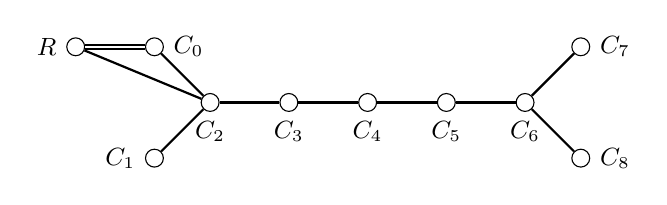
\begin{tikzpicture}
[node distance=1cm, font=\small]
\tikzstyle{vertex}=[circle, draw, fill=white, inner sep=0mm, minimum size=1.5ex]
\node[vertex]	(C2)  	at (1,0) 	[label=below:{$C_2$}] 		{};
\node[vertex]	(C3)			[right of=C2, label=below:{$C_3$}]	{};
\node[vertex]	(C4)			[right of=C3, label=below:{$C_4$}]	{};
\node[vertex]	(C5)			[right of=C4, label=below:{$C_5$}]	{};
\node[vertex]	(C6)			[right of=C5, label=below:{$C_6$}]	{};

\node[vertex]	(C7)			[above right of=C6, label=right:{$C_7$}]	{};
\node[vertex]	(C8)			[below right of=C6, label=right:{$C_8$}]	{};
\node[vertex]	(C0)			[above left  of=C2, label=right :{$C_0$}]	{};
\node[vertex]	(C1)			[below left  of=C2, label=left :{$C_1$}]	{};
\node[vertex]	(R)			[left of=C0, label=left:{$R$}]	{};

\draw [thick] (C2)--(C3)--(C4)--(C5)--(C6);
\draw [thick] (C0)--(C2)--(C1);
\draw [thick] (C7)--(C6)--(C8);
\draw [thick,double] (C0)--(R);
\draw [thick] (C2)--(R);
\end{tikzpicture}
\end{gathered}
\end{equation}
\end{proposition}

\proof
Seeking a contradiction, we assume that such a configuration exists. 
The subconfigurations  $C_0+C_1+\ldots+C_8$ and $R+C_1+\ldots+C_8$ support
curves of canonical type $\I_4^*$. Let $\varphi:Y\ra \PP^1$ and $\varphi':Y\ra\PP^1$
be the resulting genus-one fibrations. Without loss of generality we may assume
\begin{gather*}
\varphi^\inv(\infty) = C_0+C_1+2(C_2+\ldots+C_6)+C_7+C_8,\\
\varphi'^\inv(\infty) = R+C_1+2(C_2+\ldots+C_6)+C_7+C_8.
\end{gather*}
Indeed, these fibers must be simple by Proposition \ref{key reduction}, and   $\varphi^\inv(\infty)\cdot \varphi'^\inv(\infty)=4$.
Choose some half-fibers $F,F'\subset Y$ for the respective fibrations, with intersection number  $(F\cdot F')=1$.
Let $S\subset \Num(Y)$ be the subgroup generated by $C_1,\ldots,C_8,F',F$. 
As in the preceding proof, we exploit   properties of the resulting Gram matrix $N\in\Mat_{10}(\ZZ)$.
Note that this is the lattice $U\oplus D_8$, as one referee pointed out. 
% /*
%    
%    2-3-4-5-6-7
%    |       |
%    1       8
%    
%    F'= half-fiber for the orhgogonalfibration psi C_0'+C_1+...
%    F= half-fiber for original  fibration \varphi = tenth basis vector
%    We have F\cdot F'=1.
% */
% Q:=RationalField();
% Z:=IntegerRing();
% 
% N:=ScalarMatrix(10,Q!-2); N[9,9]:=0; N[10,10]:=0; 
% for i:= 1 to 6 do
% N[i,i+1]:=1; N[i+1,i]:=1;
% end for;
% N[8,6]:=1; N[6,8]:=1; 
% N[10,9]:=1; N[9,10]:=1;
% 
% N; Determinant(N); pSignature(N,-1);
% [-2  1  0  0  0  0  0  0  0  0]
% [ 1 -2  1  0  0  0  0  0  0  0]
% [ 0  1 -2  1  0  0  0  0  0  0]
% [ 0  0  1 -2  1  0  0  0  0  0]
% [ 0  0  0  1 -2  1  0  0  0  0]
% [ 0  0  0  0  1 -2  1  1  0  0]
% [ 0  0  0  0  0  1 -2  0  0  0]
% [ 0  0  0  0  0  1  0 -2  0  0]
% [ 0  0  0  0  0  0  0  0  0  1]
% [ 0  0  0  0  0  0  0  0  1  0]
% -4
% -8
%
Again    $S\subset \Num(Y)$ has index two, and the discriminant   group $A_S=S^*/S$  is elementary abelian of order four.
Recall that the inverse
\begin{equation}
\label{gram matrix second}
\source{no-enriques-surface-over-the-integers}
N^{-1}=
{\tiny
\begin{pmatrix}  
-1   &-1   &-1   &-1   &-1   &-1 &-1/2 &-1/2    &0    &0\\
-1   &-2   &-2   &-2   &-2   &-2   &-1   &-1    &0    &0\\
-1   &-2   &-3   &-3   &-3   &-3 &-3/2 &-3/2    &0    &0\\
-1   &-2   &-3   &-4   &-4   &-4   &-2   &-2    &0    &0\\
-1   &-2   &-3   &-4   &-5   &-5 &-5/2 &-5/2    &0    &0\\
-1   &-2   &-3   &-4   &-5   &-6   &-3   &-3    &0    &0\\
-1/2 &-1 &-3/2   &-2 &-5/2   &-3   &-2 &-3/2    &0    &0\\
-1/2 &-1 &-3/2   &-2 &-5/2   &-3 &-3/2   &-2    &0    &0\\
0    &0    &0    &0    &0    &0    &0    &0     &0    &1\\
0    &0    &0    &0    &0    &0    &0    &0     &1    &0\\
\end{pmatrix}
}
\end{equation}
is the Gram matrix of the induced $\QQ$-valued form on $S^*$ with respect to the dual basis $C_1^*,\ldots C_8^*,F'^*, F^*$.
% S:=N^-1;
% S;
% [  -1   -1   -1   -1   -1   -1 -1/2 -1/2    0    0]
% [  -1   -2   -2   -2   -2   -2   -1   -1    0    0]
% [  -1   -2   -3   -3   -3   -3 -3/2 -3/2    0    0]
% [  -1   -2   -3   -4   -4   -4   -2   -2    0    0]
% [  -1   -2   -3   -4   -5   -5 -5/2 -5/2    0    0]
% [  -1   -2   -3   -4   -5   -6   -3   -3    0    0]
% [-1/2   -1 -3/2   -2 -5/2   -3   -2 -3/2    0    0]
% [-1/2   -1 -3/2   -2 -5/2   -3 -3/2   -2    0    0]
% [   0    0    0    0    0    0    0    0    0    1]
% [   0    0    0    0    0    0    0    0    1    0]
The generator for the extension $S\subset\Num(Y)$   corresponds  to a non-zero isotropic vector in $A_S$, with
respect to the quadratic form $q:A_R\ra\QQ/2\ZZ$.  
Glancing at \eqref{gram matrix second}, we see that 
$$
C_1^*\equiv C_3^*\equiv C_5^*\quadand C_7^*\quadand C_8^*. 
$$
are non-zero modulo $S$,     whereas the other dual basis vectors vanish modulo  $S$, and that
$(C_1^*)^2=-1$ and $(C_7^*)^2=(C_8^*)^2=-2$. So the isotropic vectors in the discriminant group come from $C_7^*$ and $C_8^*$.
Note that   $F^*=F'$ and $F'^*=F$ belong to the sublattice $S\subset S^*$.

By Proposition \ref{key reduction}, the half fiber  $F'$ is   integral. 
We have $F'\cdot \varphi^\inv(\infty) =2$, hence $F'$ is a two-section for  $\varphi:Y\ra\PP^1$.
Let  $Y_K=\varphi^{-1}(\eta)$ be the generic fiber.
As in the preceding proof, the two-section $F'$ gives a splitting $\Pic(Y_K)=\Pic^0(Y_K)\oplus 2\ZZ$,
we get an identification $\Pic(Y_K)=\Num(Y)/S$,
and there must be another integral curve $\tilde{R}\subset Y$ that is a two-section, 
with $\Num(Y)=S+\ZZ\tR$. Furthermore, we may may assume $\tR^2=0$ or $\tR^2=-2$.
We now examine the possible non-zero intersection numbers with the components of $\varphi^\inv(\infty)$:
Since the discriminant group is annihilated by two, 
the case $(\tR\cdot C_i)=2$ with $i\in \{0,1,7,8\}$ would imply that $\tR\in S^*$ belongs to $S$, contradiction.
Also $(\tR\cdot C_i)=1$ with $i\in \{2,\ldots,6\}$ is impossible, because then $\tR$ becomes zero or non-isotropic in $A_S=S^*/S$. 
Likewise, the two cases 
$$
 (\tR\cdot C_0) = (\tR\cdot C_1) =1\quadand  (\tR\cdot C_7)=(\tR\cdot C_8)=1
$$
are impossible, because $C_0^*+C_1^*\equiv F^*+C_1^*$ and $C_7^*+C_8^*$ are non-isotropic.
Up to renumeration, the only  possibilities  left are $(\tR\cdot C_0) = (\tR\cdot C_8)=1$ and $(\tR\cdot C_1) = (\tR\cdot C_8)=1$.
If $\tR^2=-2$ then $\tR=\PP^1$ and in both cases get  a curve of canonical type $\I_8$, in contradiction to Proposition \ref{key reduction}.
Thus $\tR^2=0$, and $\tR\subset Y$ is a genus-one curve.  But then the two cases where already discarded in the proof for Proposition \ref{no I4*}.
Summing up, the configuration \eqref{I4*+R second} also does not exist.
\qed


%===========================================================
